\chapter{Comparing Devices}
To not repeat the names of the devices, the following shortening will be used: 
\begin{itemize}
    \item watch: Withings scanwatch: \ref{section:WithingsWatch}
    \item ring: Oura ring Generation 2: \ref{section:OuraRing}
\end{itemize}
\section{Research Task}
The core application allows easy access to meassurements from multiple devices in a csv format. This enables researchers to analyse the data to answer research questions. As a supplementary project task, a data analysis was performed to answer the following research question: "Do devices used (watch and ring) produce significantly different measurements for common fields?" Importantly, this is not the same as answering: "Are devices used accurate?", as that would require a much more rigorous study; that would require ground-truth measurements for every day, which are hard to acquire in practice, as those machines are expensive, non-mobile, require technician, etc. So it would be a very expensive, industry-level study, which is out of scope for this project. Instead, the precision of the differences in device measurements is examined rather than individual device's accuracy. 
\section{Data}
There are 60 days of my own personal data from both devices for every day. I always wore both devices at the same time, never one device but not the other; Both devices were configured properly - such as indicating correct weight in both apps every week and setting reference values for heart-rates to automatic. That means that data from devices is directly comparable. It is only 60 days because I acquired the ring later in the year than the watch, around the end of December, so earlier data could not be used as there is no corresponding ring data. Lastly, only common measurements were used. The only non-common measurement was REM sleep duration, which the watch does not measure, so that field was deleted from the ring's rows for the analysis.
% TODO technologies in backend.
\section{Exploration}
Python with pandas, numpy and statsModels were used for analysis. To explore the dataset, Bland-Altman plot was used on various common measurements. The difference in measurements for the same date is calculated by: $\text{ring[property]} - \text{watch[property]}$, meaning that negative values mean that the ring's measurement was lower, i.e the watch's measurement was higher.
\begin{figure}
    
    \centering
    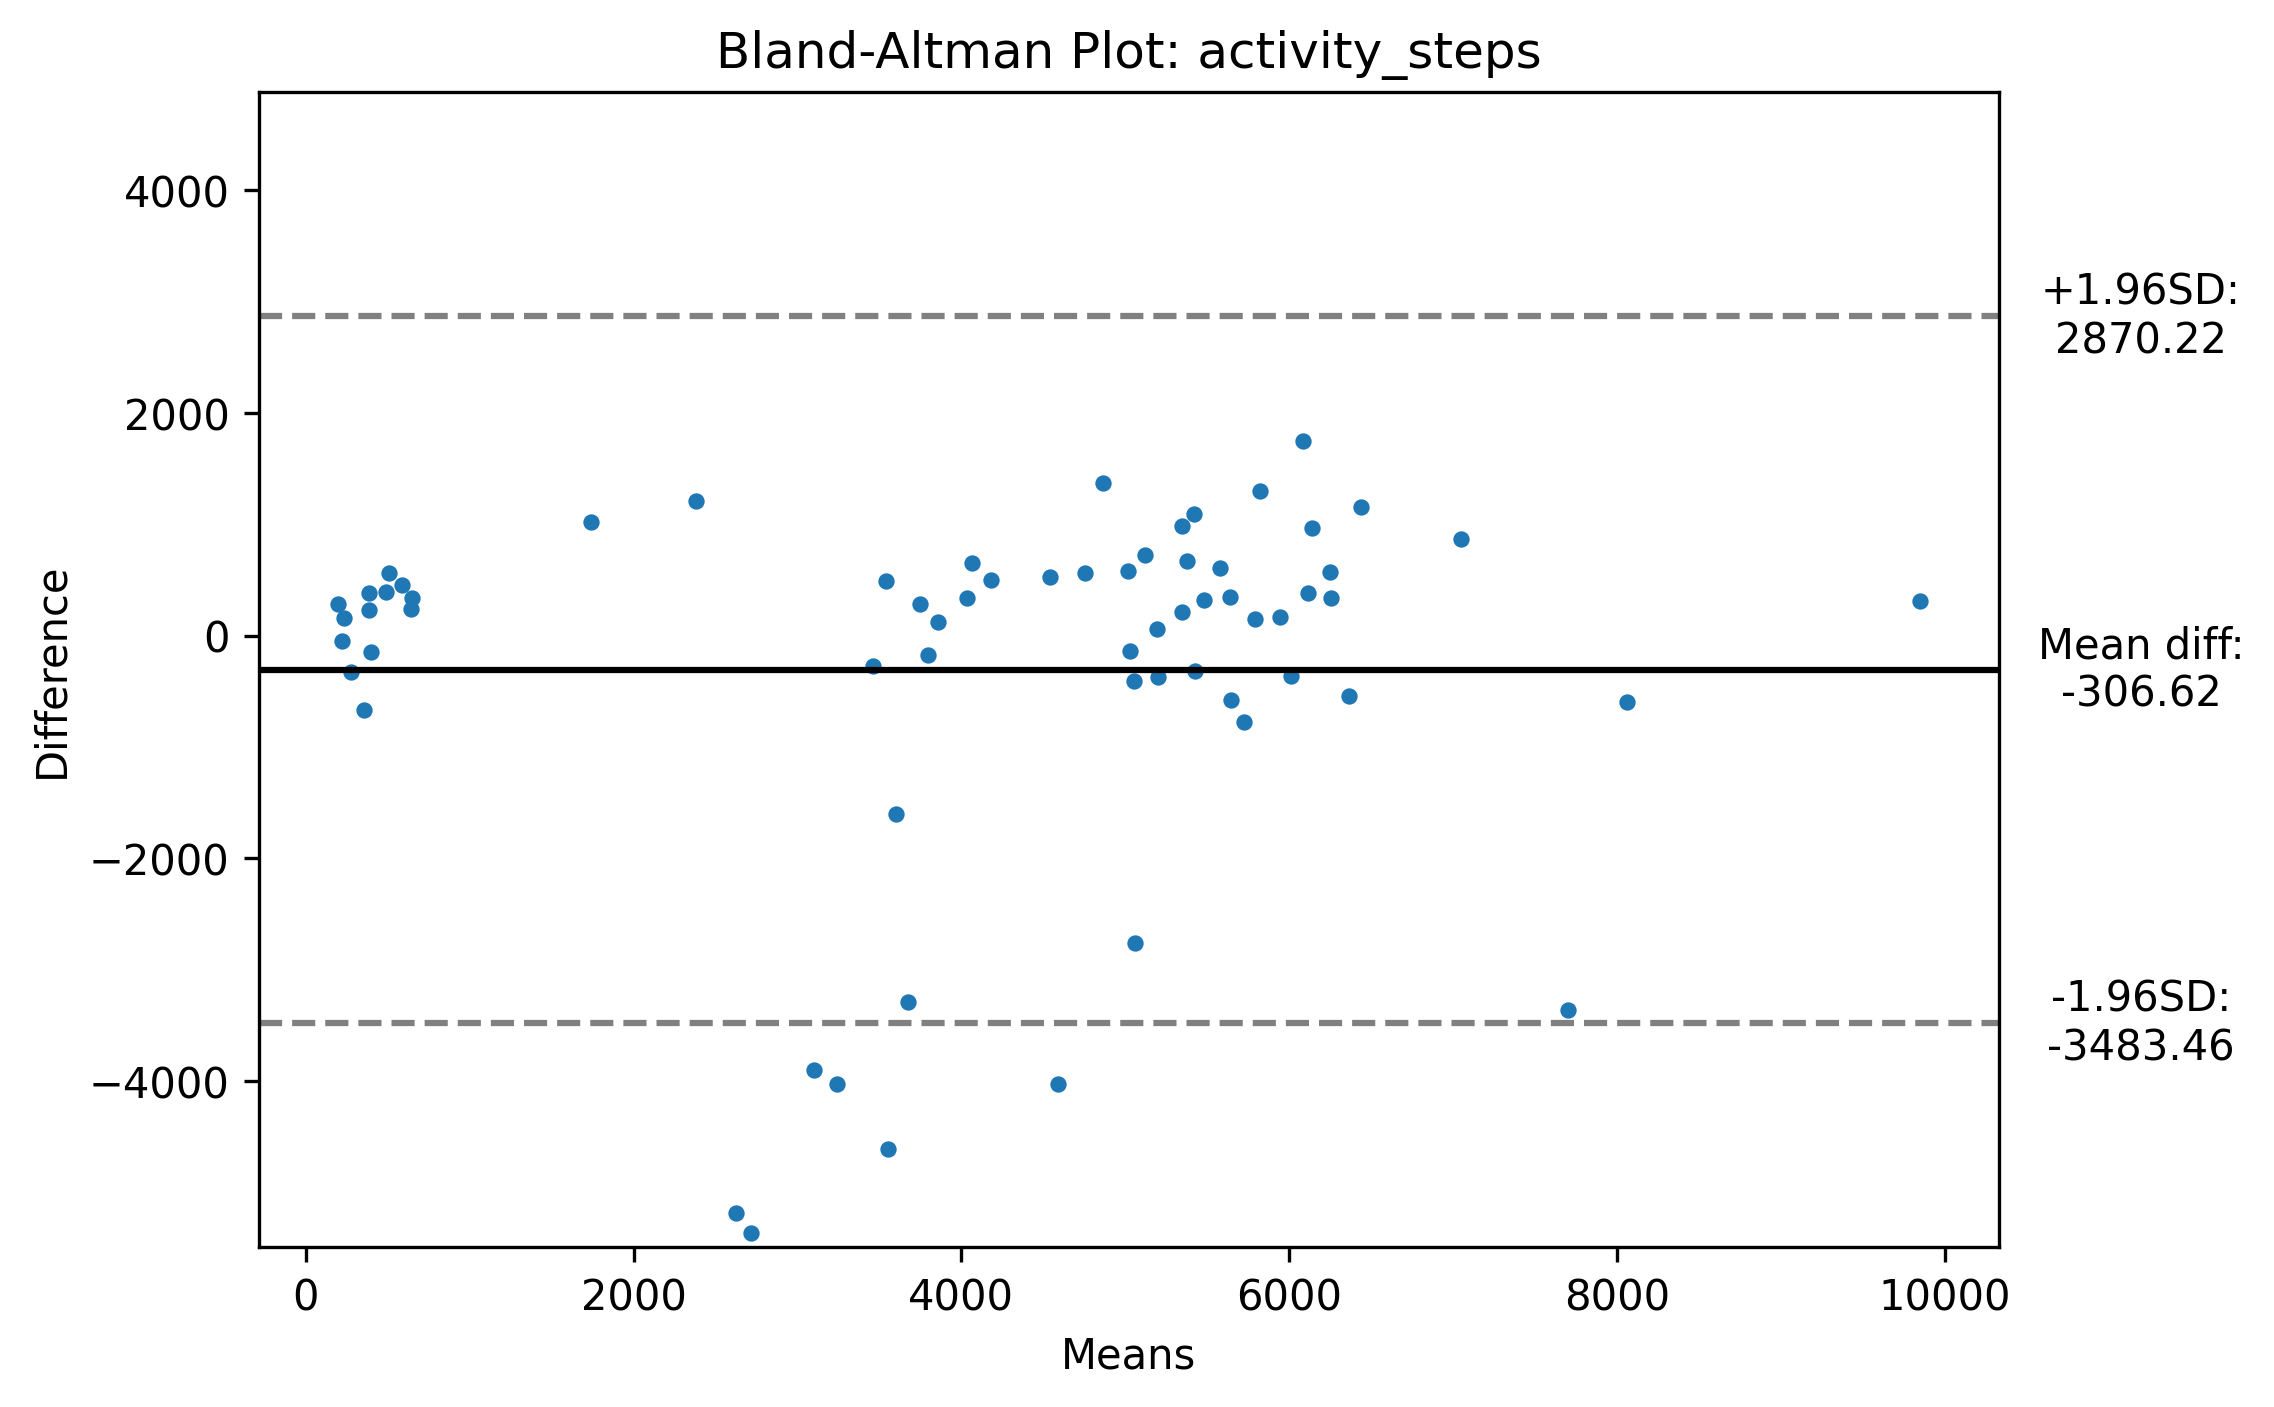
\includegraphics[width=\textwidth,keepaspectratio]{../images/bland_altman_steps.png}
    \caption{Bland-Altman Plot for Steps}
    \label{fig:blandAltmanSteps}
    
\end{figure}

For steps \ref{fig:blandAltmanSteps}, the average difference between devices is quite small, with the watch recording 306 more steps, which is a pretty small difference; for example, if the watch recorded the daily recommended number of steps - 10000, then the ring would have 9694 steps, which is only 3.06\% away from the goal. Overall there is not a lot of variability in the differences, as vertically points are mostly clustered around the mean difference line. However, the results are heavily influenced by outliers, which are unlikely to occur naturally; More than a 4000 step count difference, which is more than 2 standard deviations away, does not make much sense and is most likely due to some error. 
\begin{figure}
    
    \centering
    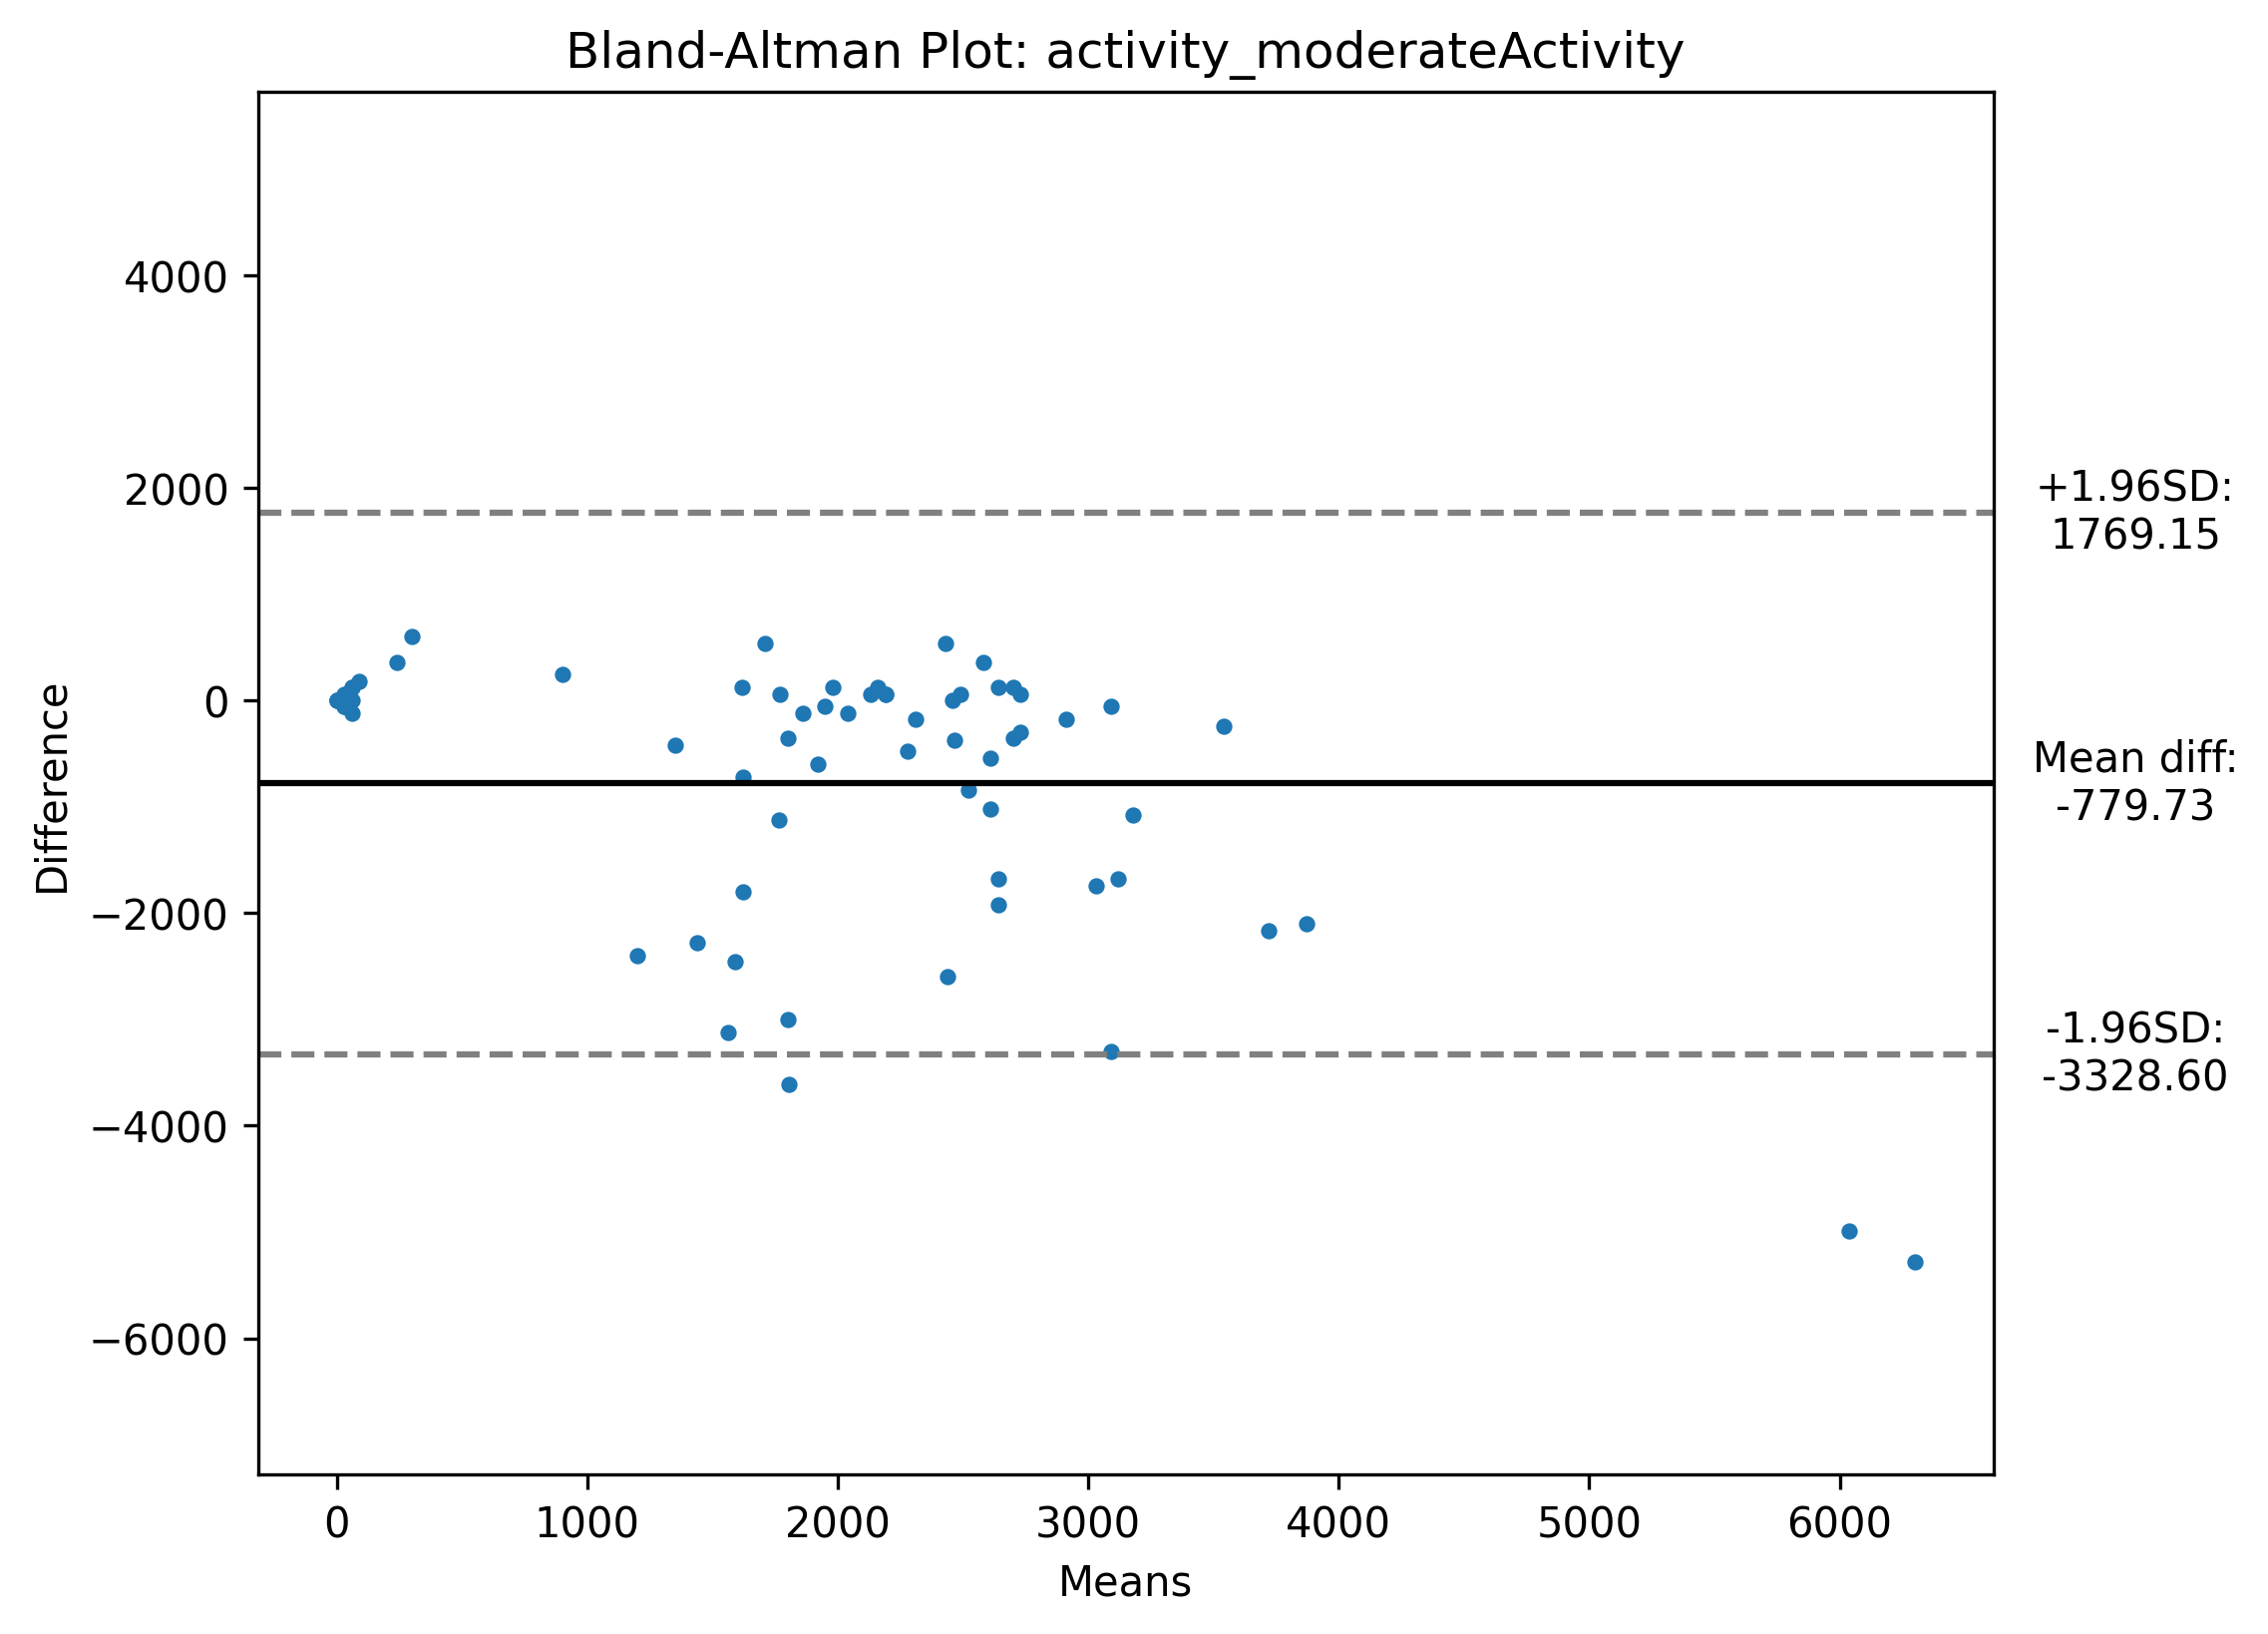
\includegraphics[width=\textwidth,keepaspectratio]{../images/bland_altman_moderateActivity.png}
    \caption{Bland-Altman Plot for Moderate Activity Seconds}
    \label{fig:blandAltmanSoftActivity}
    
\end{figure}

For moderate activity \ref{fig:blandAltmanSoftActivity}, the difference is more significant, with the watch recording 779 seconds (13 minutes) more of moderateActivity on average. Although the difference might seem small, when considering how it translates into MET minutes, it has important implications. For example, with a daily activity goal of 178 MET minutes, and using MET multiplier of 3 for moderate activity, when the watch reached the goal, the ring only recorded 139 ($178 - 13 * 3$), which is 22\% away from reaching the goal; this adds up to missing 273 MET minutes in a week. Interpretation of this depends on which device is more accurate, if watch is accurate then the ring underinflates, which is better than the other option that the ring is accurate and the watch overinflates, and of course both could be slightly away from true value; for example, assuming the ring is more accurate, users that use the watch might feel confident that they reached their activity goals with purpose of losing weight, when in fact they are missing a sizeable chunk of exercise, which could sabotage their confidence, as they might be losing less weight in reality than predicted. On a personal note, I do feel that the ring is more accurate, as I have manually timed my deliberate moderate activity time on a single day, with the watch giving 27 minutes, ring giving 18 and manual being 20.

Although care has been made to collect high quality data, there might be user errors. Sometimes the watch could have lost contact with the skin due to loose strap for comfortable wear, or some device turned off due to charge running out. Also, development of the core product was still underway, so maybe some changes caused some notifications to be lost. To combat outliers, z-scores are computed for each data point, and values that that have $-2 <= z <= 2$ are removed, i.e remove data points more than 2 stds. away. The following are Bland-Altman plots with outliers removed for the examined properties: Steps \ref{fig:blandAltmanStepsNoOutliers} and Moderate Activity \ref{fig:blandAltmanModerateActivityNoOutliers}. The difference in step count went down to 114 which is a neglible difference, whereas difference in the moderate activity remained relatively high at 10 minutes, suggesting that there is some systematic difference between devices.

\begin{figure}
    
    \centering
    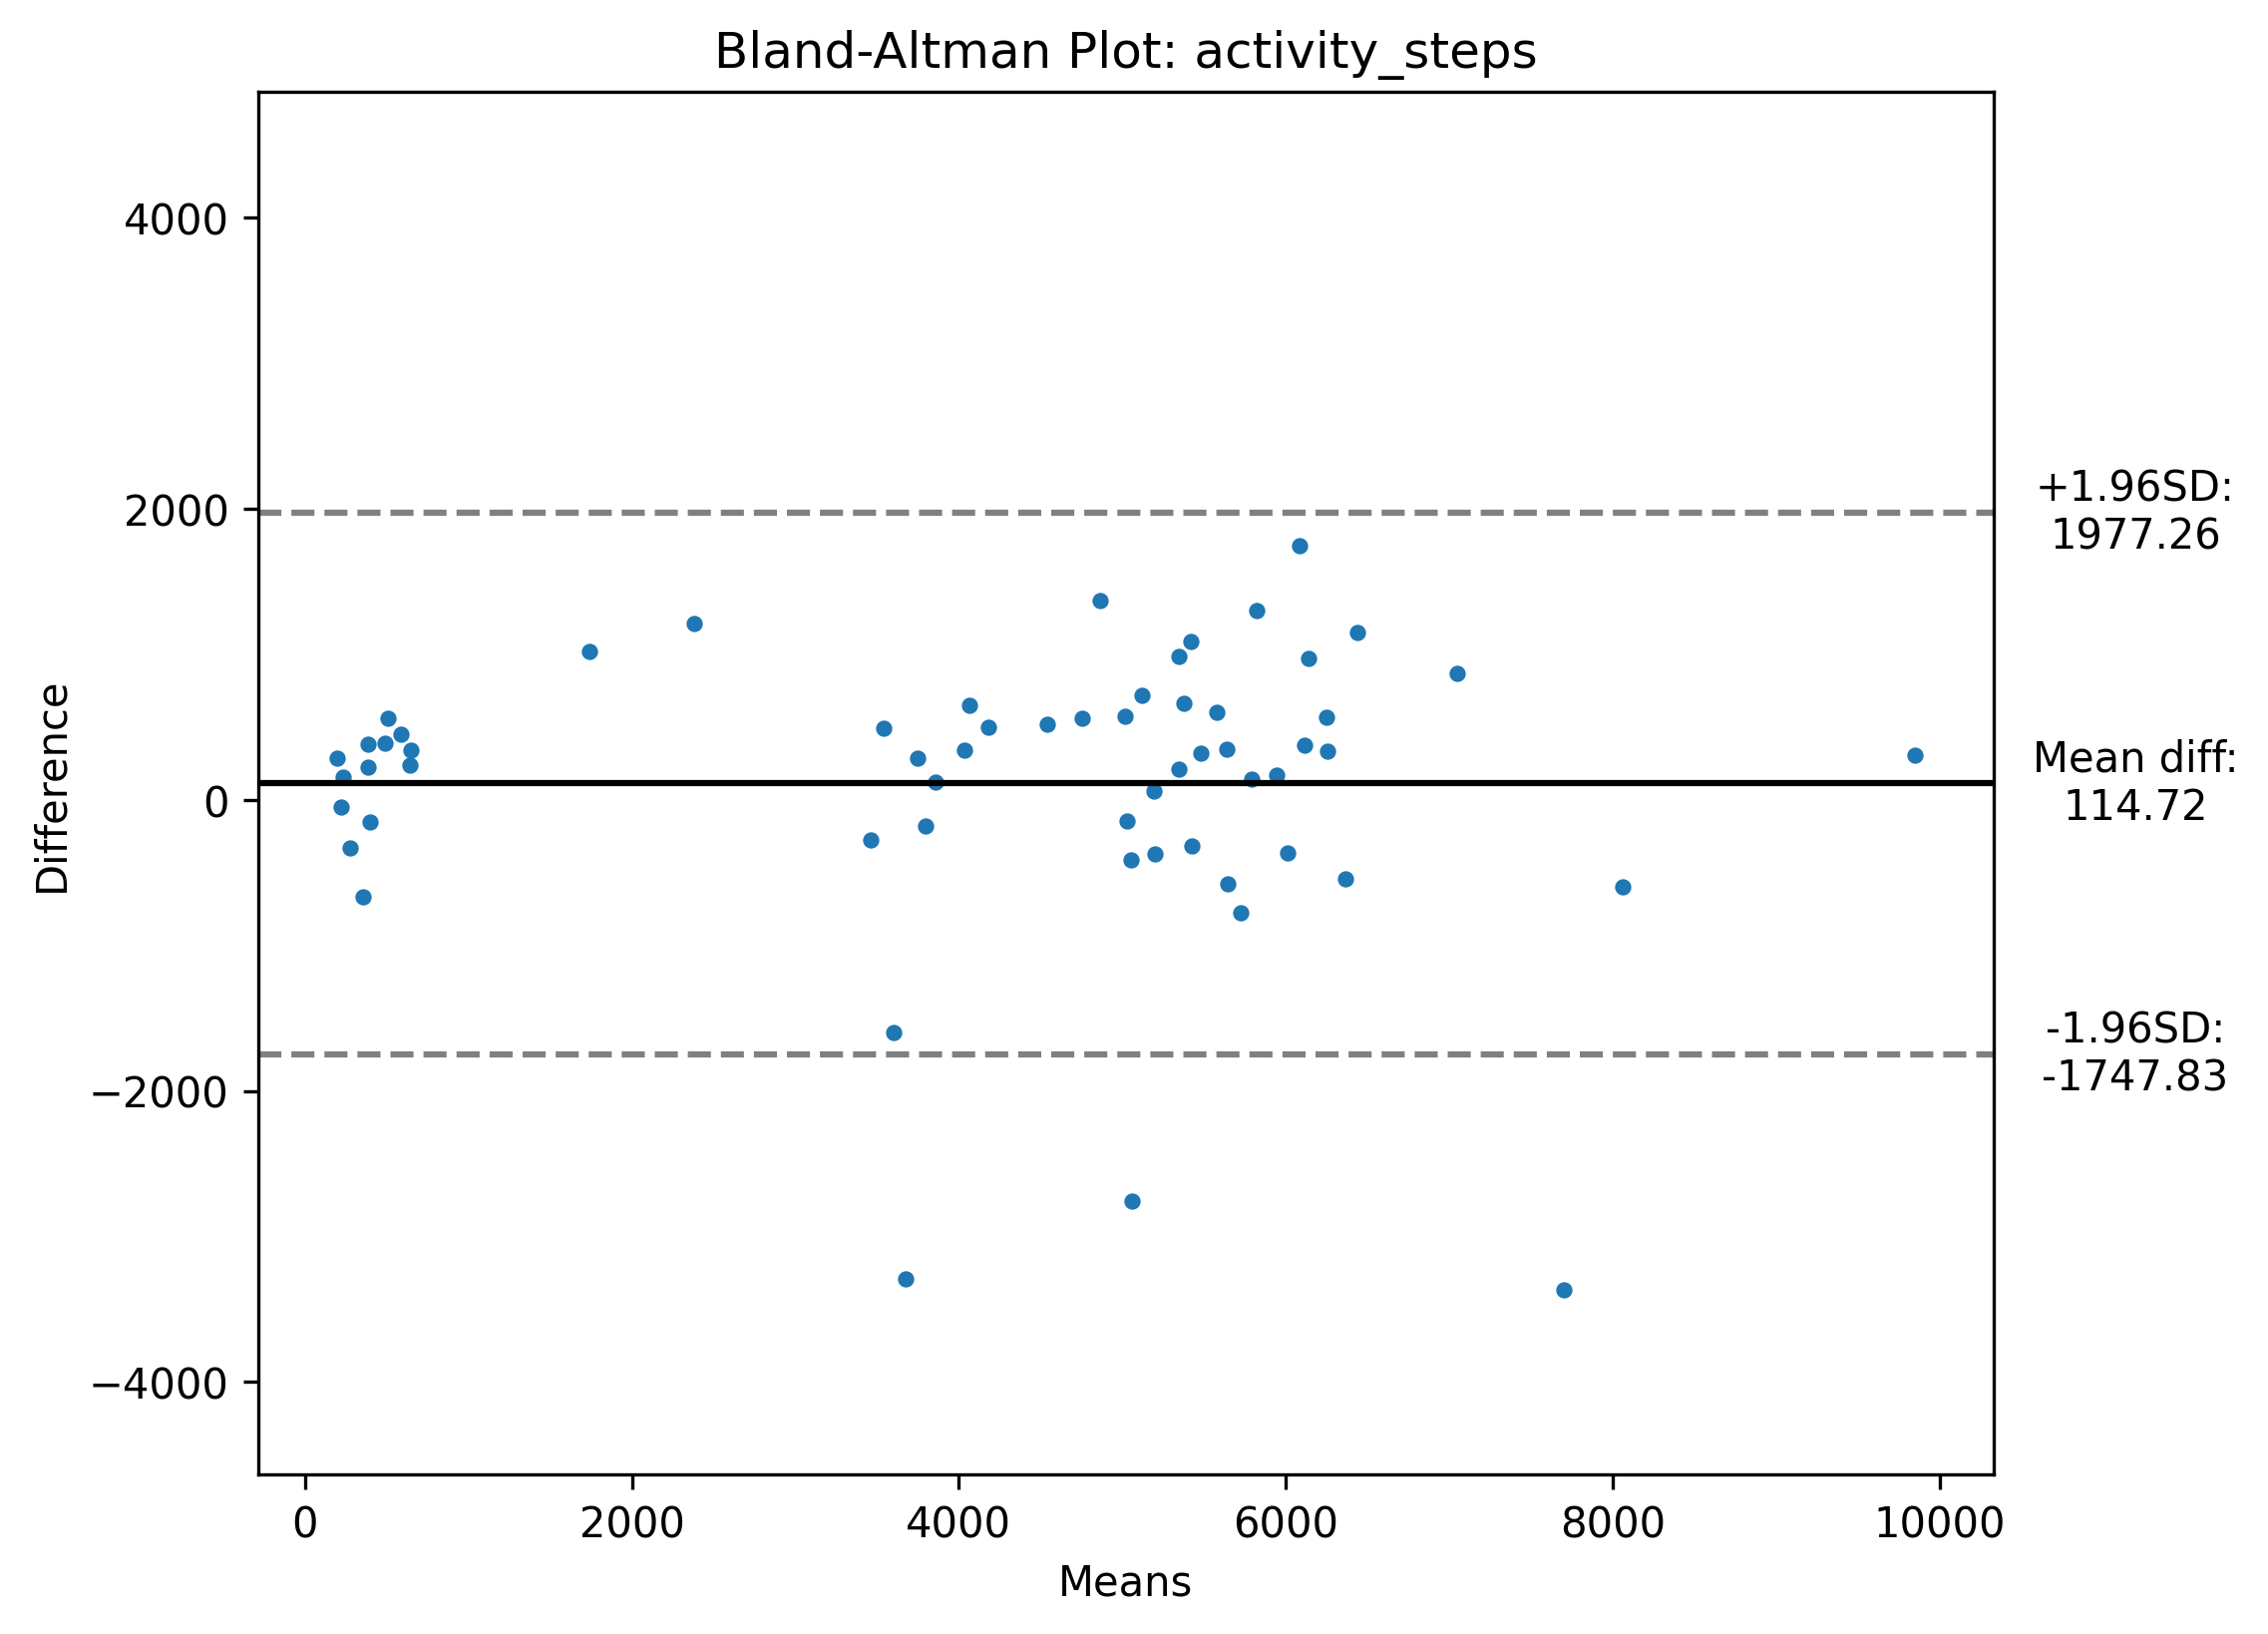
\includegraphics[width=\textwidth,keepaspectratio]{../images/bland_altman_steps_no_outliers.png}
    \caption{Bland-Altman Plot for Steps with previous outliers removed}
    \label{fig:blandAltmanStepsNoOutliers}
    
\end{figure}
\begin{figure}
    
    \centering
    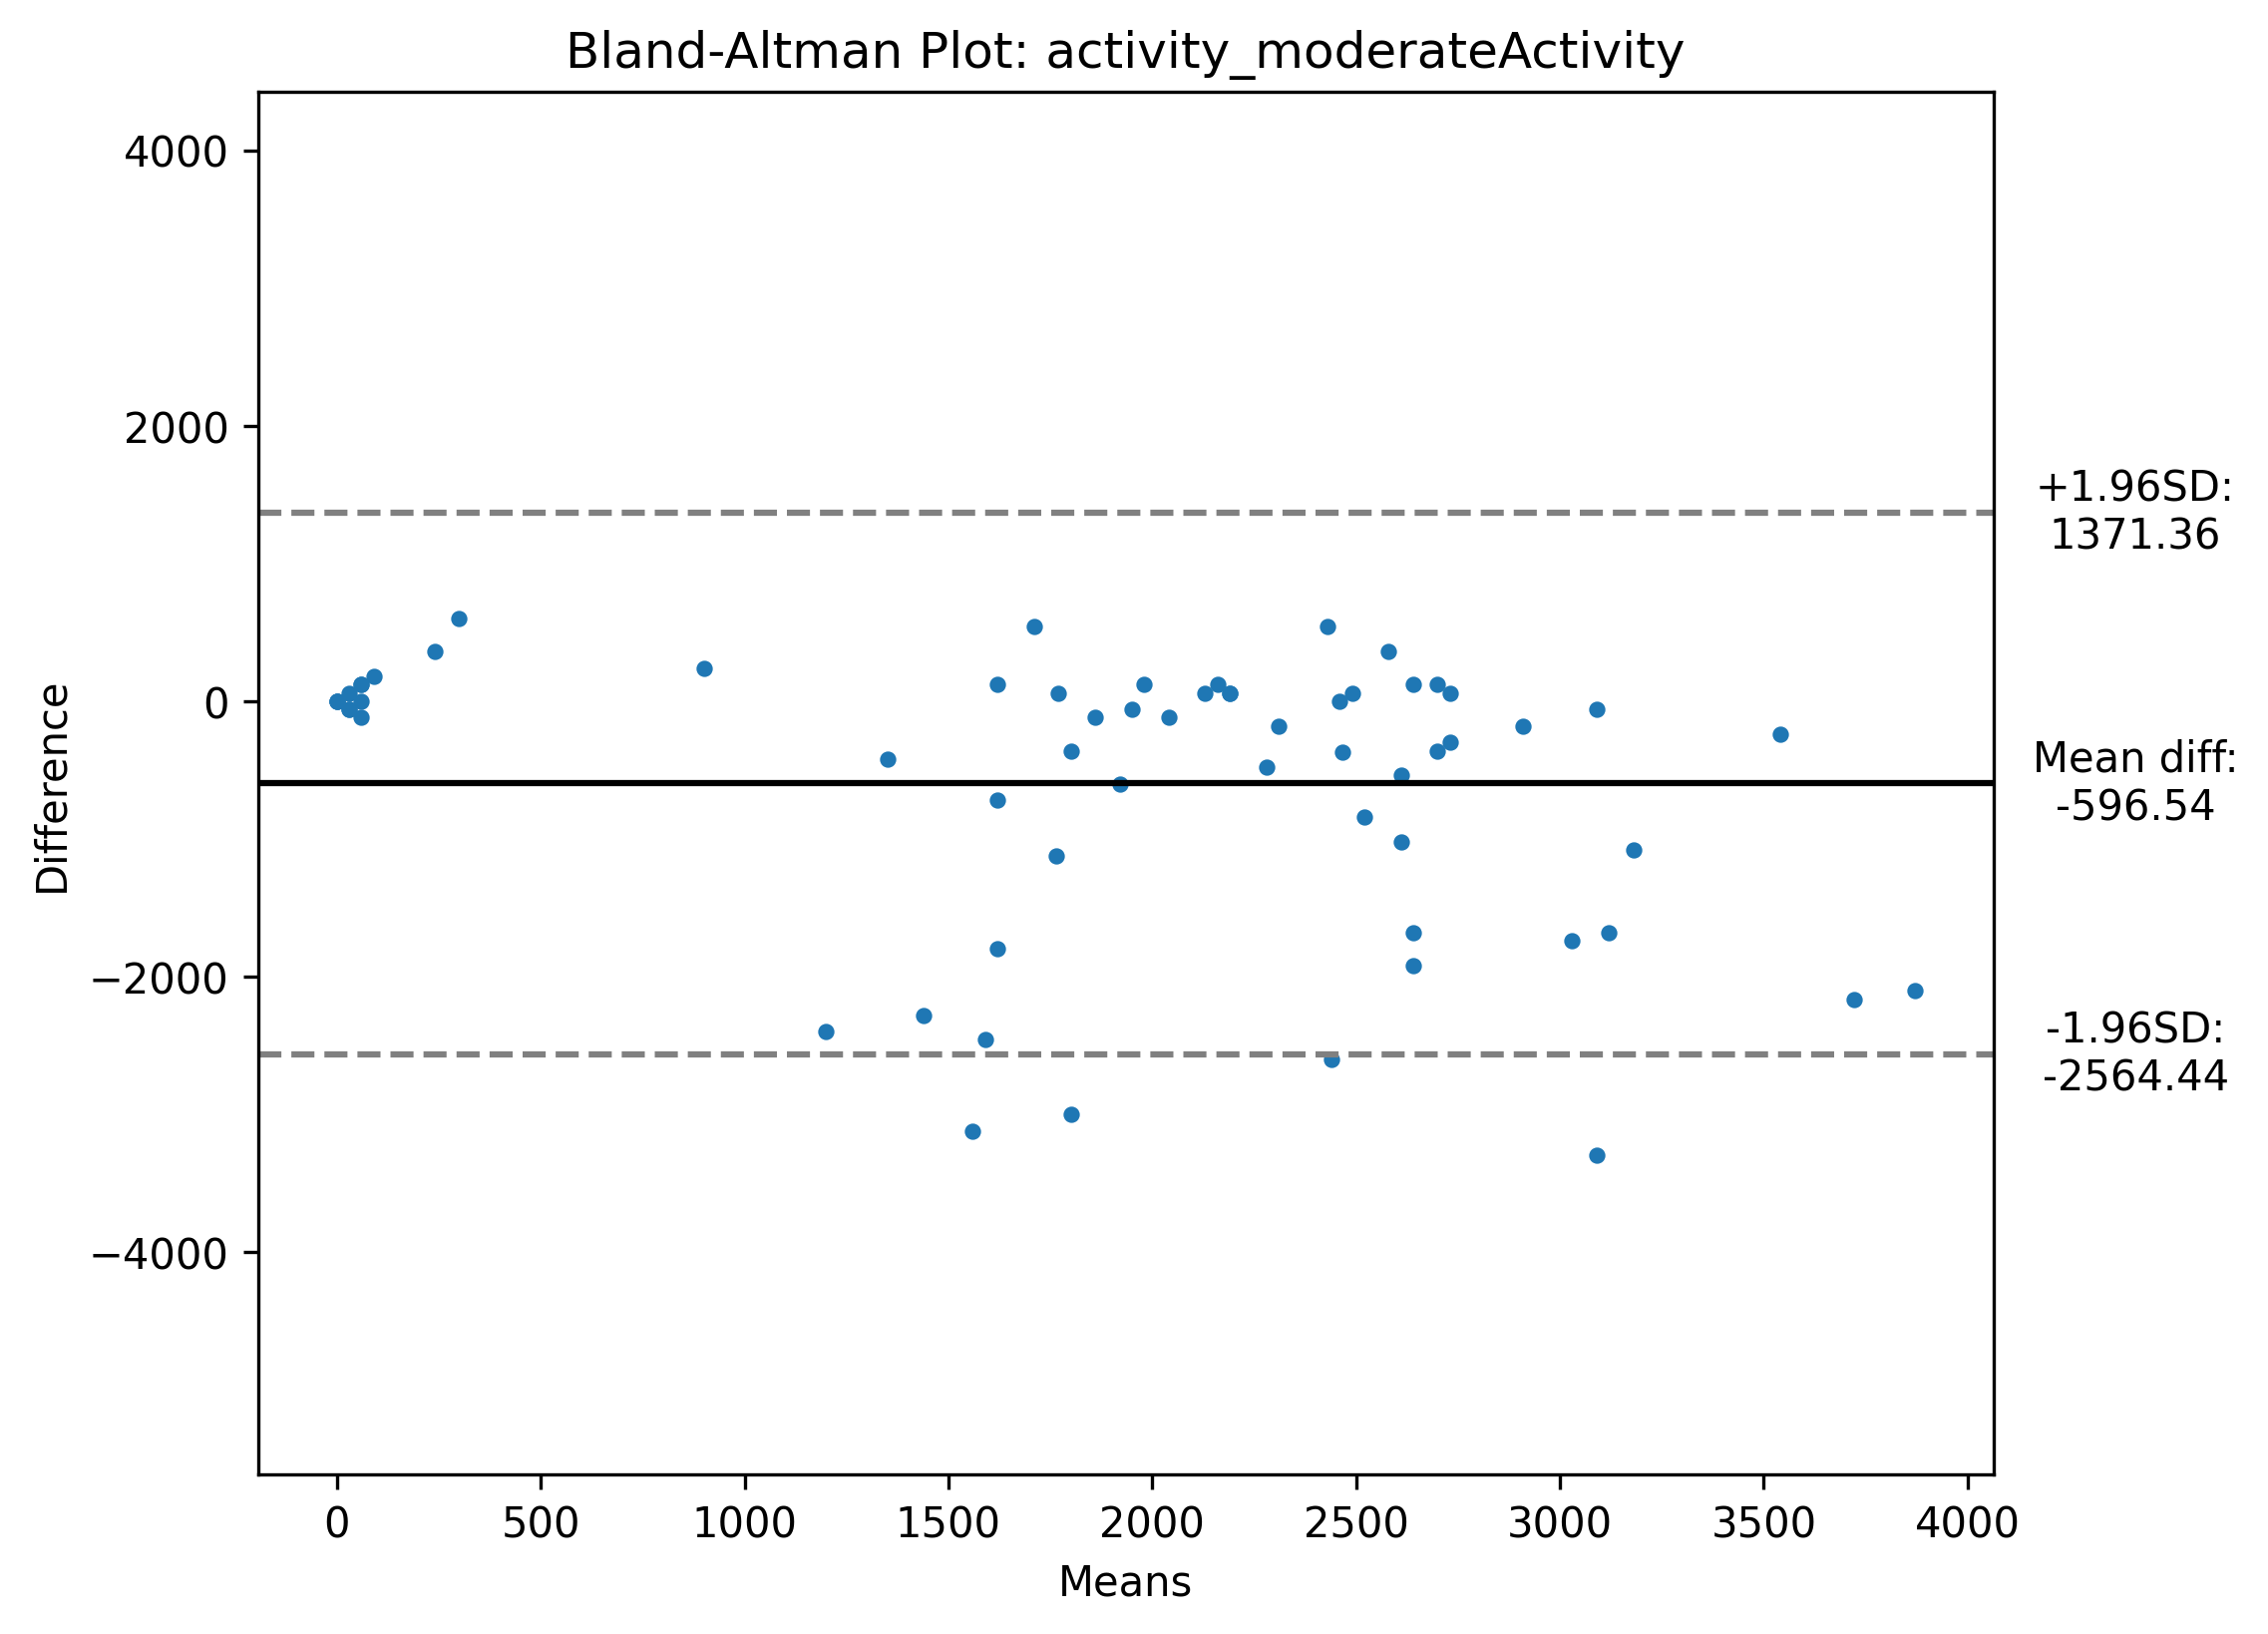
\includegraphics[width=\textwidth,keepaspectratio]{../images/bland_altman_moderateActivity_no_outliers.png}
    \caption{Bland-Altman Plot for Moderate Activity Seconds with previous outliers removed}
    \label{fig:blandAltmanModerateActivityNoOutliers}
    
\end{figure}
% TODO: background for bland altman, outlier detection - zscore, two one sided t-tests for equivalence bound, t-test.
% Lambda Region: Virginia less expensive that london. dynamo configured as provisioned minimum readers and writers.


